\documentclass[12pt,a4paper]{article}
% \usepackage{fontspec} % habilita UTF-8 nativo (solo XeLaTeX/LuaLaTeX)
\usepackage[utf8]{inputenc} % habilita UTF-8 para pdflatex
\usepackage[T1]{fontenc}    % codificación de fuente para pdflatex
\usepackage[spanish]{babel}
\usepackage{geometry}
\usepackage{setspace}
\usepackage{hyperref}
\usepackage{titlesec}
\usepackage{float}
\usepackage{graphicx} % Para insertar imágenes
\usepackage{tikz}
\usetikzlibrary{shapes,arrows,positioning,fit}


\geometry{margin=2.5cm}
\setstretch{1.3}

\titleformat{\section}{\large\bfseries}{\thesection.}{1em}{}

\begin{document}

%----------------------------------------------------------
% PORTADA
%----------------------------------------------------------
\begin{titlepage}
    \centering
    \vspace*{3cm}
    {\LARGE\textbf{Predicción de Consumo Energético en Ciudades Inteligentes}}\\[1cm]
    {\Large Proyecto de Procesamiento de Grandes Volúmenes de Datos}\\[2cm]
    {\large Autores:}\\[0.3cm]
    {\large Amalia Beatriz Valiente Hinojosa}\\
    {\large Noel Pérez Calvo}\\[1cm]    
    \vfill
\end{titlepage}

%----------------------------------------------------------
% CONTENIDO
%----------------------------------------------------------

\section{¿Qué se pretende lograr?}

El objetivo central del proyecto es \textbf{predecir el consumo energético en distintas zonas de una ciudad inteligente}, utilizando técnicas de procesamiento de grandes volúmenes de datos mediante las plataformas \textit{Hadoop} y \textit{Apache Spark}.  
A través del análisis de datos históricos de consumo eléctrico, se busca anticipar la demanda en las próximas horas, detectar picos de consumo y evaluar el impacto de las condiciones climáticas sobre el uso energético urbano.

\section{Dataset seleccionado}

\textbf{Nombre:} \textit{Household Electric Power Consumption Dataset} \\[0.2cm]
\textbf{Fuente:} Kaggle / UCI Machine Learning Repository \\[0.2cm]
\textbf{Formato:} CSV (valores separados por punto y coma “;”) \\[0.2cm]
\textbf{URL:} \href{https://www.kaggle.com/datasets/uciml/electric-power-consumption-data-set}{https://www.kaggle.com/datasets/uciml/electric-power-consumption-data-set}

\section{Justificación del dataset}

\subsection*{Volumen}
El conjunto de datos contiene más de \textbf{dos millones de registros}, correspondientes a mediciones minuto a minuto del consumo eléctrico de un hogar durante casi \textbf{cuatro años} (2006–2010).  
Su tamaño aproximado de 120 MB en formato txt, y el incremento que supone su almacenamiento distribuido en \textit{HDFS}, permiten simular un entorno realista de \textbf{procesamiento de grandes volúmenes de datos}, adecuado para la aplicación de tecnologías como \textit{Hadoop} y \textit{Spark}.

\subsection*{Características}
El dataset incluye variables como:
\begin{itemize}
    \item Fecha y hora de cada registro.
    \item Potencia activa y reactiva global.
    \item Voltaje y corriente.
    \item Energía submedida en tres zonas del hogar (\textit{Sub\_metering\_1}, \textit{2} y \textit{3}).
\end{itemize}
Estas variables conforman una \textbf{serie temporal multivariable}, adecuada para tareas de predicción y análisis de patrones de consumo.  
Además, los datos presentan una variabilidad natural y cierto nivel de ruido, lo que refleja condiciones reales de consumo y permite evaluar técnicas de limpieza y modelado robustas.

\subsection*{Pertinencia}
El conjunto de datos resulta altamente pertinente para los objetivos del proyecto, ya que:
\begin{itemize}
    \item Contiene \textbf{registros reales de consumo energético}, directamente relacionados con la meta de predecir la demanda eléctrica.
    \item Su granularidad temporal (minuto a minuto) facilita el análisis de \textbf{patrones horarios, diarios y estacionales}.
    \item Puede combinarse con datos meteorológicos (temperatura, humedad, precipitaciones) para analizar el \textbf{impacto del clima} en la demanda, fortaleciendo el enfoque de ciudades inteligentes.
\end{itemize}

\section*{Conclusión}
El dataset seleccionado constituye una base sólida para el desarrollo del proyecto, ya que ofrece volumen, calidad y relevancia suficientes para implementar un sistema de predicción energética escalable mediante herramientas de procesamiento distribuido.  
De esta manera, se busca contribuir al diseño de estrategias de eficiencia y sostenibilidad energética en el contexto de las ciudades inteligentes.

\section{Fase 1: Análisis y Definición del Productor de Datos (Producer)}

En esta primera etapa del proyecto se diseña el flujo general del componente \textit{Producer}, encargado de la generación y envío continuo de datos hacia el sistema distribuido basado en Hadoop. Este módulo simulará el flujo de información proveniente de sensores inteligentes instalados en una red eléctrica urbana.

\subsection{Objetivo del Producer}
El objetivo del \textit{Producer} es emular la llegada de mediciones energéticas en tiempo real, transmitiendo registros de consumo eléctrico hacia un sistema de mensajería (por ejemplo, Apache Kafka) que actúe como capa intermedia entre las fuentes de datos y el almacenamiento distribuido en HDFS.

De esta forma, el sistema completo podrá procesar, analizar y visualizar los datos de consumo en tiempo real, permitiendo detectar patrones de demanda, anomalías y picos de consumo en diferentes zonas de la ciudad.

\subsection{Estructura de los Datos}
Los datos utilizados provienen de un conjunto de mediciones de energía con las siguientes variables:

\begin{itemize}
    \item \textbf{Date}: Fecha de la medición (formato \texttt{YYYY-MM-DD}).
    \item \textbf{Time}: Hora exacta de la medición (formato \texttt{HH:MM:SS}).
    \item \textbf{Global\_active\_power}: Potencia activa global (kW).
    \item \textbf{Global\_reactive\_power}: Potencia reactiva global (kW).
    \item \textbf{Voltage}: Voltaje promedio (V).
    \item \textbf{Global\_intensity}: Intensidad de corriente (A).
    \item \textbf{Sub\_metering\_1}: Consumo energético parcial del área 1 (Wh).
    \item \textbf{Sub\_metering\_2}: Consumo energético parcial del área 2 (Wh).
    \item \textbf{Sub\_metering\_3}: Consumo energético parcial del área 3 (Wh).
\end{itemize}

Estas variables reflejan el comportamiento energético de una vivienda o conjunto de zonas urbanas a lo largo del tiempo y permiten realizar análisis tanto locales como agregados sobre la red eléctrica.

\subsection{Frecuencia de Envío}
El flujo de simulación definido enviará una lectura cada \textbf{0.5 segundos}, representando un ritmo razonable para la actualización continua de datos de consumo en una red inteligente. Cada mensaje incluirá un único registro (una fila del dataset) en formato JSON o CSV, con su respectivo sello temporal.

\subsection{Flujo de Datos}
El flujo del \textit{Producer} seguirá las siguientes etapas:
\begin{enumerate}
    \item \textbf{Lectura de datos}: el módulo leerá progresivamente las filas del dataset energético.
    \item \textbf{Estructuración}: cada fila será convertida en un mensaje estructurado, conteniendo los campos definidos y un timestamp.
    \item \textbf{Emisión periódica}: cada 5 segundos, el \textit{Producer} enviará el siguiente mensaje al sistema de mensajería (Kafka).
    \item \textbf{Transporte distribuido}: los mensajes se propagarán a través de los tópicos de Kafka, permitiendo su consumo por distintos módulos del sistema (almacenamiento en HDFS, análisis en Spark, visualización, etc.).
\end{enumerate}


\subsection{Diagrama del Flujo de Datos del Producer}

\begin{figure}[H]
    \centering
    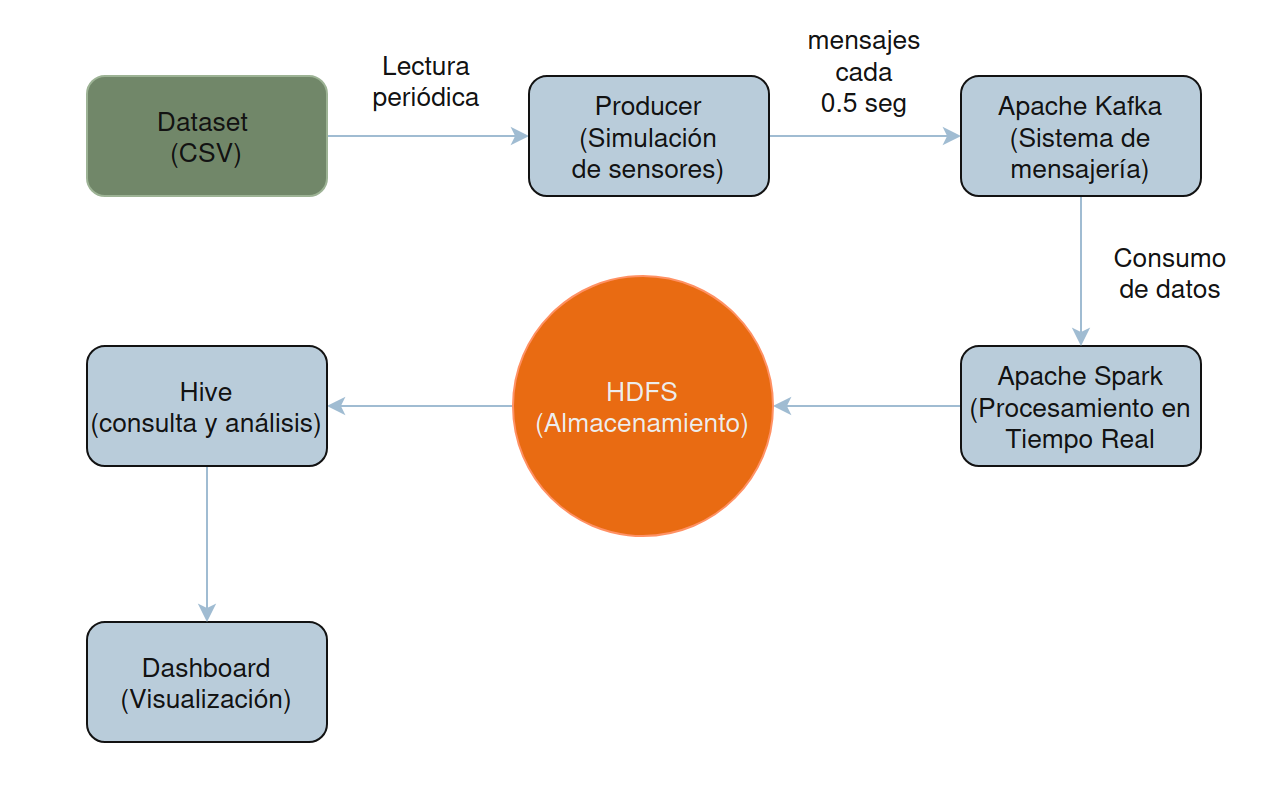
\includegraphics[width=0.9\textwidth]{diagram.png}
    \caption{Flujo general del Producer dentro del sistema distribuido basado en Hadoop.}
\end{figure}

\section{Fase 2: Implementación del Entorno Distribuido con Docker}

En esta fase se procede al diseño e implementación del entorno de ejecución distribuido que permitirá la interacción entre los distintos componentes del sistema. Para lograr un entorno reproducible y escalable, se utiliza \textbf{Docker} como herramienta de contenedorización y orquestación.

\subsection{Objetivo de la Fase}
El objetivo principal de esta fase es levantar un entorno funcional que permita la comunicación entre el \textit{Producer} y el sistema de mensajería \textbf{Apache Kafka}, dentro de un entorno controlado y portable. Este entorno servirá como base para el procesamiento de grandes volúmenes de datos sobre la plataforma Hadoop.

\subsection{Componentes del Entorno}

El ecosistema de servicios a desplegar mediante Docker estará compuesto por los siguientes contenedores:

\begin{itemize}
    \item \textbf{Zookeeper:} servicio de coordinación y gestión de clústeres necesario para el correcto funcionamiento de Kafka.
    \item \textbf{Kafka Broker:} sistema de mensajería distribuido encargado de recibir, almacenar y distribuir los mensajes provenientes del \textit{Producer}.
    \item \textbf{Producer:} aplicación desarrollada en Python que leerá los datos del dataset energético y los enviará a Kafka con una frecuencia de 5 segundos por mensaje.
\end{itemize}

Cada contenedor se comunicará dentro de una misma red interna de Docker, permitiendo que el flujo de datos se mantenga encapsulado y fácilmente replicable en distintos entornos.

\subsection{Arquitectura del Entorno Docker}

El despliegue se realizará utilizando un archivo \texttt{docker-compose.yml}, que permitirá definir los servicios y sus relaciones.  
El esquema de comunicación entre los contenedores se muestra en la Figura~\ref{fig:docker-arch}.

\begin{figure}[H]
\centering
\begin{tikzpicture}[
    node distance=2.2cm,
    every node/.style={font=\small},
    service/.style={rectangle, rounded corners, draw=blue!60, fill=blue!10, thick, minimum width=3.2cm, minimum height=1.1cm, align=center},
    producer/.style={rectangle, rounded corners, draw=orange!70!black, fill=orange!10, thick, minimum width=3.2cm, minimum height=1.1cm, align=center},
    arrow/.style={thick,->,>=stealth}
]
% NODOS EN VERTICAL
\node[service] (zookeeper) {Zookeeper};
\node[service, below of=zookeeper] (kafka) {Kafka Broker};
\node[producer, below of=kafka] (producer) {Python Producer};

% CONEXIONES
\draw[arrow] (zookeeper) -- node[right]{coordinacion} (kafka);
\draw[arrow] (producer) -- node[left]{envio de datos cada 5s} (kafka);
% RED DOCKER (marco alrededor)
\node[draw=gray!60, dashed, fit=(zookeeper)(kafka)(producer), label={[gray]below:{\textbf{Red interna Docker:} kafka-net}}, inner sep=0.5cm] {};

\end{tikzpicture}
\caption{Arquitectura lógica del entorno Docker para la simulación de datos energéticos.}
\label{fig:docker-arch}
\end{figure}

\subsection{Configuración de los Servicios}
En la práctica, la definición de los servicios en el archivo \texttt{docker-compose.yml} permitirá establecer:
\begin{itemize}
    \item Los nombres y roles de cada contenedor (por ejemplo, \texttt{zookeeper}, \texttt{kafka}, \texttt{producer}).
    \item Las redes de comunicación internas (\texttt{kafka-net}).
    \item Los puertos expuestos (por ejemplo, \texttt{9092} para Kafka y \texttt{2181} para Zookeeper).
    \item Las variables de entorno requeridas por Kafka y Zookeeper para inicializar correctamente el clúster.
\end{itemize}

\subsection{Resultados Esperados}
Al finalizar esta fase, se espera haber logrado:
\begin{itemize}
    \item Un entorno completamente funcional con Kafka y Zookeeper ejecutándose en contenedores Docker.
    \item Un contenedor adicional preparado para ejecutar el \textit{Producer} que enviará los datos simulados.
    \item Conectividad validada entre el \textit{Producer} y el Kafka Broker mediante la red interna del entorno Docker.
\end{itemize}

Este entorno constituye la infraestructura base sobre la cual se implementará el flujo de datos en tiempo real y el almacenamiento distribuido en fases posteriores.


\end{document}
